\chapter {Outras ferramentas}

\section{Grafana}

\textbf{Grafana} é uma ferramenta \textit{open-source} de monitorização \cite{Grafana}.
Esta ferramenta destaca-se pela sua interface UI muito interativa, apresentando vários gráficos e \textit{gauges}.
Deste modo, é possível criar dashboards muitos customizáveis e dinâmicas.

Ao contrário do Nagios e do Zabbix, este software é desenvolvido com um backend em \textit{Go Lang}, uma linguagem mais recente e \textit{higher-level} que \textit{C Lang}.

Devido a ser uma ferramenta gráfica poderosa, é utilizada em complemento com ferramentas mais específicas mas não tão gráficas como o Zabbix, fornecendo assim informação high-level diretamente ao utilizador.

\begin{figure}[H]
    \centering
    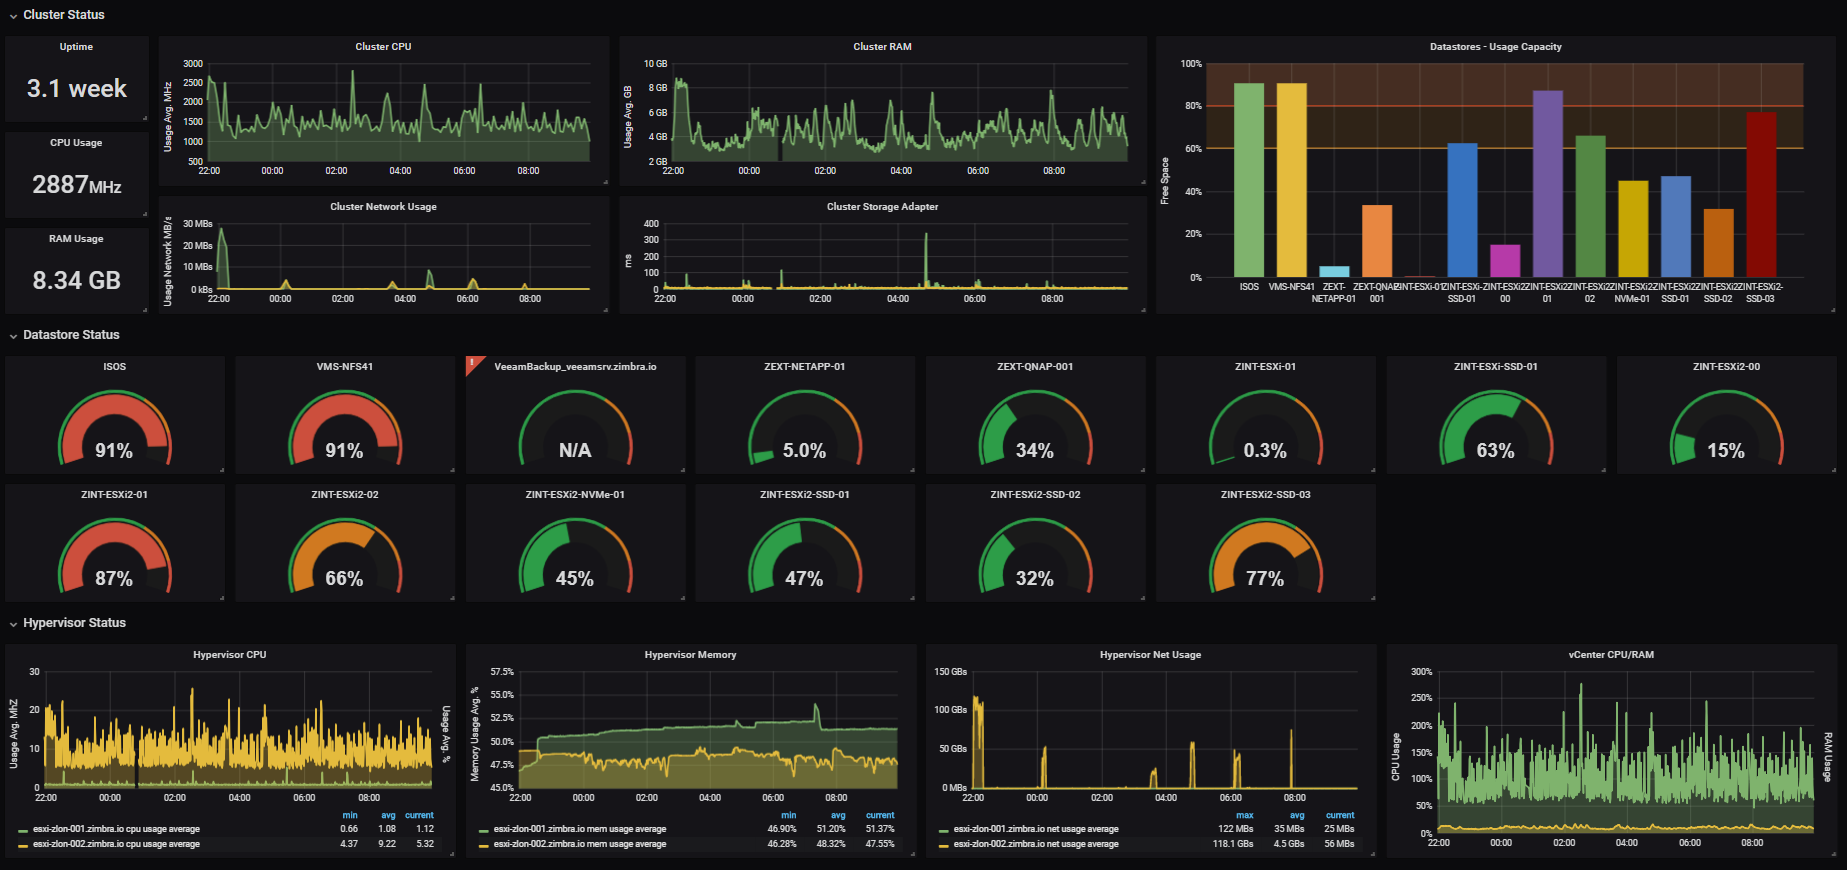
\includegraphics[width=\linewidth]{figs/others/grafana}
    \caption{UI do Grafana}
    \label{fig:grafana}
\end{figure}

\pagebreak

\section{openDCIM}

\textbf{openDCIM} é outra ferramenta de monitorização \textit{open-source} orientada para \textit{data centers} \cite{openDCIM}.
De facto, DCIM significa \textit{Data Center Infrastructure Management}.
É uma ferramenta mais específica, guardando informação relativa ao próprio hardware, sendo possível registar todo o inventário de equipamentos.
É possível também realizar testes da própria infraestrutura de rede, simulando por exemplo um corte de energia e analisando os serviços afetados.

No entanto, a UI dessa desta ferramenta é muito mais simples e mais antiga, não sendo possível ter uma interface gráfica customizável como por exemplo com o Grafana.
Disponibiliza também menos ferramentas de análise de serviços do que as outras opções.

\begin{figure}[H]
    \centering
    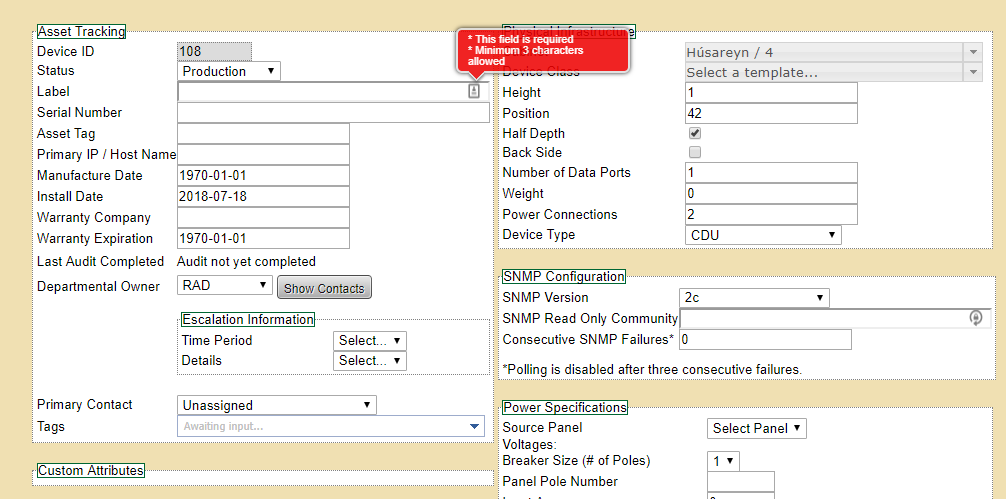
\includegraphics[width=\linewidth]{figs/others/opendcim}
    \caption{UI do openDCIM}
    \label{fig:opendcim}
\end{figure}


